\subsection{Method} \label{subsec:method_linear_regression}

Consider that we have a data set of inputs and their corresponding output. Regression is a process of arriving at a relation between the independent input variables and the dependent output variables. In the field of statistical learning, regression is considered to be a supervised learning method. This is because the model parameters generated in regression are learned from labeled data which is data that comprises both inputs and their corresponding output, i.e the labels. In this report, we assume that there are multiple input variables and a single output variable for each member of the data set.
\newline \newline
The dataset with $n$ members is defined as $\mathcal{D} := [({x}_1, y_1 ), ({x}_2, y_2 ), ..., ({x}_n, y_n )]$. Where ${x}_i$ and $y_i$  are the $i^{th}$ input and output respectively. Let, $m$ be the number of components of the input such that ${x}_i := (x_{i1}, x_{i2}, ..., x_{im})$. In linear regression we assume that the data is of the form
\begin{equation}
    {y}_i = 1 \cdot\beta_0 + x_{i1}\beta_1 + x_{i2}\beta_2 + ... + x_{im}\beta_m + \epsilon_i \label{eq:lin_reg_data}
\end{equation}
where $\beta_0, \beta_1, \dots, \beta_m$ are unknown fixed regression parameters and $\epsilon_i$ is a random error or noise process consisting of independent identically (iid) normally distributed variables with mean zero and variance $\sigma^2$ \cite{shumway_time_2017}. Equation \ref{eq:lin_reg_data} can be rewritten as $y=\beta \phi(x) + \epsilon$ with
\begin{equation}
    \phi(x):=[1, x_{i,1}, x_{i,2}, \dots, x_{i,m}].
\end{equation}
Moreover, it can be shown that $\mathbb{E}[y] = \beta \phi(x)$ and $var(y) = \sigma^2$. Therefore, $y \sim \mathcal{N}(\beta \phi(x),\,\sigma^{2})$ \cite{murphy_machine_2012}.
\newline \newline
In linear regression, we seek to fit a best-fit line between input, or some transformation of the input, and the output. This best-fit line is chosen such that it minimizes an error or a cost function. The best fit line is a function of input variables and its value is called the predicted value or the fit. We denote this with $\hat{y}$. The linear regression model has the form:
\begin{equation}
    \hat{y}_i = 1 \cdot\beta_0 + x_{i1}\beta_1 + x_{i2}\beta_2 + ... + x_{im}\beta_m
\end{equation}
The $\beta$'s are chosen such that they minimize a cost function. If this cost function is chosen to be the mean squared error (MSE) then we call the regression \textit{least squares} regression. The mean squared error is defined as 
\begin{equation}
    \mathcal{C} = \frac{1}{n}\sum_{i=1}^{n}(y_i-\hat{y}_i)^2 \label{eq:cost_function_sum}
\end{equation}

By extending the input such that ${x}_i = (1_i, x_{i1}, x_{i2}, ..., x_{im})$, i.e. the first entry of $x_i$ is a vector which only contains 1, and denoting the parameter vector by ${\beta} = (\beta_0, \beta_1, ..., \beta_m)$, we can express the predicted value as an inner product such that   
\begin{equation*}
    \hat{y}_i = {x_i}\cdot {\beta} = {x_i}^T{\beta}.
\end{equation*}
Moreover, we can express the set of predicted outputs as a vector which allows us to write the previous equation as a matrix-vector product:
\begin{equation}
    \hat{y} = {X}{\beta} \label{eq:lin_reg_matrix_model}
\end{equation}
where, $\hat{y}$, ${X}$ and ${\beta}$ have dimensions $n \times 1$, $n \times (m+1)$ and $(m+1) \times 1$. $X$ is called design matrix. However, such a description is only useful if the output is a linear or near-linear function of the input variables.  We can make the model more "complex" by allowing higher powers of input variables and their products to be the features. One possibility is to consider polynomial functions of the input variables. For simplicity, we consider input vectors where $m=2$ as they are the only ones relevant for this project. Then, we can express the predicted output $\hat{y}$ as a polynomial function of order $p$ such that
\begin{equation}
    \hat{y}_i = \beta_0 + \sum_{k=1}^{k=p}\sum_{l=0}^{l=p}\beta_{\frac{k(k+1)}{2}+l}x_{i1}^{p-l}x_{i2}^{l}
\end{equation}
which is equivalent to
\begin{equation}
\resizebox{.9\hsize}{!}{$
    \underbrace{\begin{bmatrix}y_1 \\ y_2 \\ \vdots \\ y_n\end{bmatrix}}_{n \times 1} = \underbrace{\begin{bmatrix} 
    1 & x_{11} & x_{12} & x_{11}^2 & \dots & x_{11}^p & x_{11}^{p-1}x_{12} & \dots & x_{11}x_{12}^{p-1} & x_{12}^p 
    \\ 1 & x_{21} & x_{22} & x_{21}^2 & \dots & x_{21}^p & x_{21}^{p-1}x_{22} & \dots & x_{21}x_{22}^{p-1} & x_{22}^p 
    \\ \vdots &&&&& \ddots &&&&\vdots \\ 
    1 & x_{n1} & x_{n2} & x_{n1}^2 & \dots & x_{n1}^p & x_{n1}^{p-1}x_{n2} & ... & x_{n1}x_{n2}^{p-1} & x_{n2}^p
    \end{bmatrix}}_{n \times \frac{p^2+5p}{2}}\underbrace{\begin{bmatrix}\beta_0 \\ \beta_1 \\ \vdots \\ \beta_{\frac{p^2+3p}{2}}\end{bmatrix}.}_{\frac{p^2+5p}{2} \times 1}$}
\end{equation}
For clarity if $p=2$
\begin{equation*}
    \hat{y}_i = \beta_0+\beta_1 x_{i1} + \beta_2 x_{i2}.
\end{equation*}
We see that the output vector is linear in the vector of parameters even though it is nonlinear in the features. Note that $p$ determines the model complexity and therefore the number of columns in the design matrix and the number of parameters. The output vector though depends only on the number of inputs. By changing $p$ we are changing the basis with which we describe $y_i$. 
\newline \newline
As mentioned before our aim is to find $\beta$ such that the cost function is minimized. We start by rewriting the equation \ref{eq:cost_function_sum}:
\begin{equation}
    \mathcal{C}(\beta) = \frac{1}{n}\sum_{i=1}^{n}(y_i-\hat{y}_i(\beta))^2 = \frac{1}{n}( y -  {\hat y})^T( y -  {\hat y}) = \frac{1}{n}( y -  {X\beta})^T( y -  {X\beta}).
\end{equation}

The cost function is at its minimum when its gradient with respect to all parameters is 0, i.e.
\begin{equation*}
    \nabla_{\beta}\mathcal{C}(\beta) = X^T(y-X\beta) = 0.
\end{equation*}

Assuming that $X$ has full column rank, and hence $X^T X$ is positive definite, solving the above equation provides us with the optimal parameters as follows
\begin{equation}
    \beta = (X^TX)^{-1}X^Ty.
\end{equation}
The cost function for a linear regression problem is convex. Hence, there is only one global extremum. This is not proven in this report.
\newline \newline
In the case where $X^T X$ is near singular or singular calculating the pseudoinverse (specifically the
Moore-Penrose inverse) is a very useful and well-known method. It calculates the inverse by using the Singular Value Decomposition algorithm. Moreover, this approach is more efficient than computing the regular inverse \cite{geron_hands-machine_2019}.
\newline \newline
An important step when calculating the best suited model for given input and output data is the splitting of the dataset $\mathcal{D}$ into a training dataset $\mathcal{D}_{train} = \{\boldsymbol{x}_{train}, y_{train}\}$ and a test dataset $\mathcal{D}_{test} = \{\boldsymbol{x}_{test}, y_{test}\}$. The ratio of the number of data points in the $\mathcal{D}_{test}$ to the number of data points in the $\mathcal{D}_{train}$ is called the test ratio $r$. The model parameters are learned on the training dataset in the training phase. While, the performance of the model is assessed by various indicators that compare the output of fitting the model, on the input of the test set, with the output of the test set. \newline

Let the mean squared error(MSE) be 
\begin{equation}
    MSE(y, \hat{y}) = \frac{1}{n}\sum_{i=1}^{n}(y_i - \hat{y_i})^2
\end{equation}
the squaring is important so that the positive and negative errors do not cancel each other. Certainly, the lower the value of MSE the closer is our prediction($\hat{y}$) to the ground truth($y$). The training MSE is given as $MSE_{train} = MSE(y_{train}, \hat{y}_{train})$ and the testing MSE as $MSE_{test} = MSE(y_{test}, \hat{y}_{test})$. 

The MSE can be decomposed into bias and variance as 
\begin{equation}
    MSE = \underbrace{\mathbb{E}[(y - \mathbb{E}[\hat{y}])^2]}_{\text{bias}} + \underbrace{\mathbb{E}[(\hat{y} - \mathbb{E}[\hat{y}])^2]}_{\text{variance}} + \sigma^2
\end{equation}

Let the $R^2$ score be 
\begin{equation}
    R^2(y, \hat{y}) = 1 - \frac{\sum_{i=1}^{n}(y_i-\hat{y})^2}{\sum_{i=1}^{n}(y_i-\mathbb{E}[\hat{y}])^2}.
\end{equation} 
It measures the ability of the model to capture the true variance relative to the actual variance. When the model fits the data perfectly $R^2=1$. While, the least possible value of $R^2_{train}$ is 0, but $R^2_{test}$ can be negative.  

The difference in the MSE values  for the training and testing set determines the degree of generalization of the model from trained data to new unseen data. The average generalization error is \cite{mehta2019high}
\begin{equation*}
    |MSE_{train} - MSE_{test}| = 2\sigma^2\frac{m}{n}.
\end{equation*}
If $m >> n$ then the model is not generalising, i.e. learning. In addition, the error can be large if the intrinsic noise $\sigma^2$ in the data is large. To counter this problem, regularisation is performed. In regularisation, the parameter values are penalized. In ridge regression, the $L^2$ norm of the parameter vector is penalized and in lasso regression, the $L^1$ norm of the parameter vector is penalized. This is done by modifying the cost functions as follows
\begin{align}
    \mathcal{C}_{ridge}(\beta) &=  \frac{1}{n}( y -  {X\beta})^T( y -  {X\beta}) + \lambda||\beta||_2^2, \\
    \mathcal{C}_{lasso}(\beta) &=  \frac{1}{n}( y -  {X\beta})^T( y -  {X\beta}) + \lambda||\beta||_1.
\end{align}

\subsubsection{Feature Scaling}\label{subsubsec:scaling}
In general, machine learning algorithms do not perform well if the scales of the data vary a lot. There exist different scaling methods. We focus on min-max scaling, also known as min-max normalization. In this approach, the values are scaled and shifted such that they range from 0 to 1, i.e. 
\begin{equation*}
    x^{'} = \frac{x - min(x)}{max(x) - min(x)}.
\end{equation*}

\subsubsection{Need for resampling}
Typically, data contains outliers. These outliers can be erroneously obtained data. They can also be the true data that sometimes deviates from the established patterns of the system due to intrinsic noise. The presence of outliers in both the training and the testing set can either influence the fitting of parameters or the statistics. Therefore, it is essential to subdue the effects of outliers using methods that usually involve multiple iterations of training and testing on different subsets of the data. Moreover, the statistics obtained for a single fit are not necessarily the true indicator of the model performance. There is intrinsic variance in those statistics. To ameliorate the effect of variance we utilize resampling techniques. In resampling, we repeatedly learn the model with a different training set and find their statistical performance on the different test sets. In the end, the mean of the statistics of individual iterations is taken to be the final statistic. \newline \newline In the following sections we discuss two of the most commonly used methods: the bootstrap algorithm and cross-validation. 
\subsubsection{Bootstrap Algorithm}\label{subsubsec:bootstrap}
The bootstrap algorithm is a resampling technique that uses sampling with replacement. There are multiple variants of the bootstrap method. We use one that is distinct from the lecture notes. \newline
The steps of the algorithm are as follows:
\begin{enumerate}
    \item Let the number of bootstrap iterations on given data be: $n_{boots}$
    \item For each bootstrap iteration $n_{bi}$:
    \begin{enumerate}
        \item Randomly divide the input data consisting of $n$ samples into two categories. The two categories are the training and test set. The training set has $(1-r)n$  number of samples which are randomly selected with replacement. The rest of the samples then make up the testing set. Therefore the number of samples in the testing set is greater than or equal to $rn$. Here, $r$ is the testing ratio.
        \item Train parameters for the training set and fit them to the testing set.
        \item Compute statistics on the training set: $MSE_i, R^2_i$
    \end{enumerate}
    \item The final statistics of the bootstrap algorithm are the mean of the statistics of all the bootstrap iterations.
\end{enumerate}

\begin{figure}[H]
    \centering
    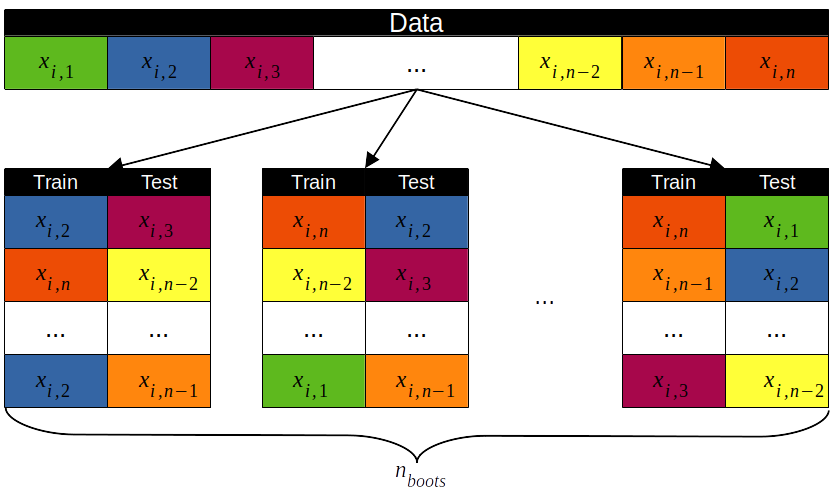
\includegraphics[width=1\linewidth]{Images/bootstrap_diagram.png}
    \caption{Flowchart of the bootstrap algorithm.}
    \label{fig:bootstrap_algorithm}
\end{figure}

\subsubsection{K-fold Cross-Validation}\label{subsubsec:cross_validation}
K-fold cross-validation is an ideal method to circumvent the problem that data is often scarce and there is usually not enough data to set aside a validation set. To avoid this problem the data into $k$ parts of the same size \cite{friedman2001elements}. \newline
The steps of the algorithm are as follows:
\begin{enumerate}
    \item The data is divided into a finite number $k_{folds}$ of equal-sized sets called folds.
    \item For each fold $k_{fi}$:
    \begin{enumerate}
        \item Take the fold as the testing set while the rest of the folds comprise the training set.
        \item Train parameters for the training set and fit them to the testing set.
        \item Compute statistics on the training set: $MSE_i, R^2_i$
    \end{enumerate}
    \item The final statistics of the cross-validation algorithm are the mean of the statistics obtained by considering each fold as the testing set.
\end{enumerate}
\begin{figure}[H]
    \centering
    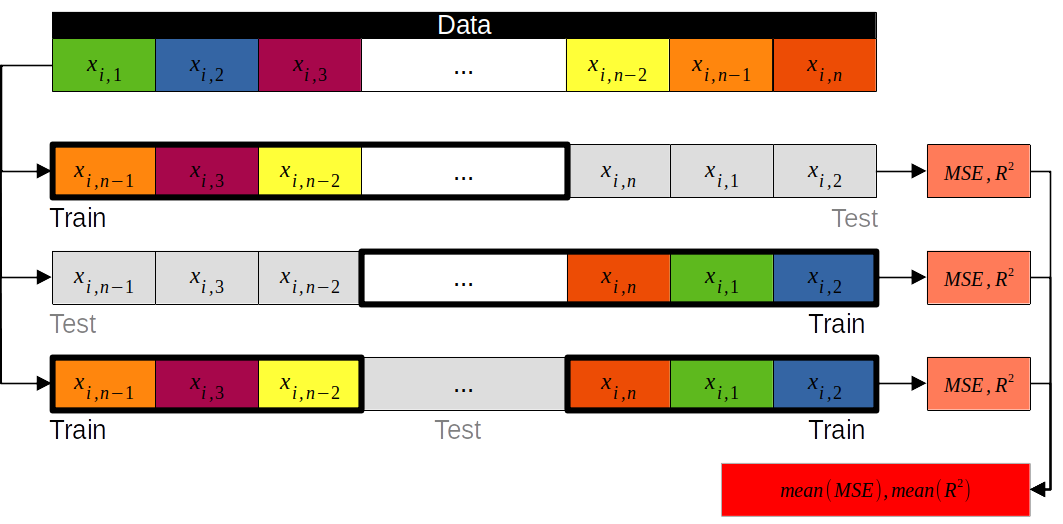
\includegraphics[width=1\linewidth]{Images/cross_validation_diagram.png}
    \caption{Flowchart of the k-fold cross-validation algorithm with $k_{folds}=3$ and $n=9$.}
    \label{fig:cross_val_algorithm}
\end{figure}

%\subsubsection{Stochastic Gradient Descent}\label{subsubsec:SGD}
%SGD is not a machine learning technique but an optimization technique. It is useful in the optimization %requirement for logistic regression. 

%SGD comes in various variants. The most common variant due to its good empirical performance is a mix of epoch and mini-batches. Mini-batches are a subset of data of size m obtained by sampling the whole training data without replacement. This is where randomness and stochasticity come from.